%                                             -*- coding: utf-8 -*-
% Mindenkinek csak javasolni tudjuk, hogy latex-et használjon.
% Szakdolgozatnál vagy diplománál már egyértelműen kijönnek az
% előnyei a Worddel szemben.  Ennek ellenére ez a sablon messze nem
% tökéletes.
% Ha valamit javítanál benne, kérlek, küld vissza, hogy
% hallgatótársaid is profitáljanak belőle.  Köszönöm.
% További nehézséget okoz, hogy a népszerű latex disztribúciók nem
% tartalmazzák a legújabb változatát a magyar.ldf-nek.
% A szükséges
% fájlokat a sablon mellé bemásoltuk, de le is tölthetőek innen:
% http://www.math.bme.hu/latex/
%
%
%
\documentclass[a4paper,oneside]{article}
\usepackage[margin=3cm]{geometry}
% =================================================================
% Magyar nyelvi támogatás
%------------------------
% ###################
% Nyelvváltó parancsok:
%\selectlanguage{english}
%\selectlanguage{magyar}
% rövid angol beszúrás:  \foreignlanguage{english}{some english text}
% határozott névelők generálása ``magyar'' babel-el:
% argumentum+megfelelő határozott nevelő: \az{},\Az{}
% csak a megfelelő határozott nevelő: \az*{}, \Az*{}
% címkék: \aref{}, \aref*{}, képletekhez \aref()
%        \Aref{}, \Aref*{}, képletekhez \Aref()
% oldalak: \apageref{}, \apageref*{}
%        \Apageref{}, \Apageref*{}
% idézetek: \acite, \acite*, \Acite, \Acite*
% ###################
\usepackage[english,magyar]{babel} %vegyes nyelvi támogatás a
% magyar helyesírás ellenőrzéshez (ispell) és elválasztáshoz
\selectlanguage{magyar}

%=================================================================
% direkt ékezetes karakter beírás támogatás
%-------------------------------------------
\usepackage[T1]{fontenc}
\usepackage[utf8]{inputenc}
\usepackage{multirow}
\usepackage{booktabs}
%================================================================
% Undorító dolog bitmappelt (Type III) betűtípust nézni a 
% PDF-ben
% képernyőn. Az alapértelmezett Computer Modern font LaTex-ben
% bitmappelt, ezért használjunk Times fontot:
\usepackage{times}

%================================================================
% ha ábrát akarunk beemelni, akkor használjuk a graphicx/graphics
% csomagot és az \includegraphics[width=<width>]{abra.pdf} parancsot
\usepackage{graphicx} %for graphics
\usepackage{subcaption}
\usepackage{placeins}
\usepackage{tikz}
\usetikzlibrary{positioning, arrows.meta}
%kepek helye a gyokerhez(ehhez a file-hoz kepest) kepest
\graphicspath{{./figs/}}

%================================================================
% Kötelezően használjuk a hyperref csomagot, mert ezzel többek között 
%  kulturált hyperlinkelt PDF-et lehet csinálni az alábbi
%  variációkban, különféle hyperref backend-ekkel:
%  pdflatex,dvipdfm,ps2pdf
% tapasztalataim szerint a MikTeX (Win32) a 'dvipdfm' konverzióval
% optimális  míg a teTeX (Linux/Solaris) jobb szereti a 'dvips' módszert
%------------------------------------
% pontosan egyet kommentezzünk be!!!!!!!
% értelemszerűen backend függően generáljunk dvi-ból PDF-et!!!
%------------------------------------
% A hyperref csomag az utolsó beolvasott csomag legyen, kivéve néhány
% problémás csomagot, pl.
% algorithm
%-----------
% ########################### FONTOS ###########################
% A hyperref hibásan működik a babel csomag 'magyar.ldf' fájljának
% 1.5-ös verziójánál korábbi változatával.
% 2004. februárjában a MikTeX
% és teTex disztribúciók még csak a v.1.4 verziót tartalmazták!
% A fájl
% aktuális verziója a BME Matematikai intézet LaTeX honlapjáról
% elérhető: http://www.math.bme.hu/latex/ 
% A lusták kedvéért a jelen sablon mellé is mellékelem:
% magyarlatex_0.01-2.tar.gz 
% ########################### FONTOS ###########################
%-----------
\usepackage[colorlinks=true]{hyperref}

\setcounter{topnumber}{2}
\setcounter{bottomnumber}{2}
\setcounter{totalnumber}{4}
\renewcommand{\topfraction}{0.9}
\renewcommand{\bottomfraction}{0.8}
\renewcommand{\textfraction}{0.08}
\renewcommand{\floatpagefraction}{0.85}
\setlength{\textfloatsep}{10pt plus 2pt minus 2pt}

%%%%%%%%%%%%%%%%%%%%%%%%%%%%%%%%%%%%%%%%%%%%%%%%%%%%%%%%%%%%%%%%%%%
% Itt kezdődik maga a dokumentum
%%%%%%%%%%%%%%%%%%%%%%%%%%%%%%%%%%%%%%%%%%%%%%%%%%%%%%%%%%%%%%%%%%
\begin{document}
\input{onlabmacros} % Ez kell!!!
\markright{Pálos Ferenc (U1OTPN)} % egyoldalas fejléc!!!
%--------------------------------------------------------------------
% fedlap
%--------------------------------------------------------------------
\begin{titlepage}
%bme logo 
 \begin{figure}[h]
    \centering
      
\includegraphics[width=12cm]{bme_logo}
  \label{fig:bme_logo}
  \end{figure}
  \thispagestyle{empty}
  %cím generálás
  \onlabcim

 \begin{center}
   \begin{tabular}{ p{3cm} p{5cm} }
   
   Készítette: & Pálos Ferenc  \\
   Neptun-kód: & U1OTPN  \\
   Szakirány: & Mérnökinformatika, Intelligens hálózatok  \\
   E-mail cím: & palosferenc@proton.me  \\
   Konzulens: & Dr. Ladóczki Bence  \\
   E-mail cím: & ladoczki.bence@vik.bme.hu  \\%   
   \end{tabular}
 \end{center}

 
  
%\feladatcim argumentuma a feladat rövid, 1 soros címe
    \feladatcim{Weboldal-ujjlenyomat-készítés (website fingerprinting) vizsgálata Tor hálózaton} 

  %\feladatmaga argumentuma a feladat 1-2 bekezdésnyi ismertetése
  \feladatmaga{A Tor egy népszerű anonimizáló hálózat, amely napi több millió felhasználó adatvédelmét szolgálja önkéntesek által üzemeltetett proxyk (köztes átjátszó szerverek) segítségével.
Célja, hogy elrejtse a kommunikáció forrását és célját, védve a felhasználókat a megfigyeléstől és a cenzúrától.
Az anonimitást fenyegető egyik legjelentősebb támadási forma a weboldal-ujjlenyomat-készítés (website fingerprinting, WF), amely során a támadó a Tor hálózatba való belépési pont forgalmából következtethet a meglátogatott oldalakra.
A projekt célja annak vizsgálata, hogy a WF támadások mekkora valós fenyegetést jelentenek a Tor felhasználóira, és hogy különböző forgalmi környezetekben – normál Tor forgalomban (baseline) és obfs4 pluggable transport (forgalom-elfedő modul) mellett –, illetve ismeretlen webhelyekkel bővített (nyílt világú) beállításban hogyan változik a gépi tanulási modellek teljesítménye.
Ennek részeként elvárás a valós forgalmi minták gyűjtése szimulált környezetben, etikus keretek között, az adatok előkészítése a gépi tanuláshoz, valamint egy egységes jellemzőtér és a top-10 leginformatívabb jellemző kiválasztási stratégiájának kialakítása az alkalmazott modellcsaládok teljesítményének összehasonlíthatósága érdekében.
A munka második részeként két eltérő megközelítés kidolgozása és kiértékelése szükséges: egy klasszikus gépi tanulási megoldás (Random Forest) és egy reprezentáció-tanuláson alapuló architektúra (Triplet MLP + KNN), amely egy tanult beágyazási téren alkalmaz KNN osztályozást.
A kiértékelésnek egységes metrikákkal (pontosság, macro-F1) és az eredmények grafikus ábrázolásával kell történnie.
A tanítási és tesztelési adatok eloszlás-eltolódását (domain shift), amely a baseline és az obfs4 adatok közti különbségből adódik, valamint a zero-shot beállítások hatását – ahol a betanítás és a tesztelés eltérő környezetben történik – szintén számszerűsíteni kell.}

 
  %\tanevfelev argumentumok:
  % #1=Tanév (xxxx/xx alakban), #2=félév (pont nélkül!)
  
  \tanevfelev{2025/26}{II}
 
\end{titlepage} 

\setcounter{page}{2}

%==================================================================
\section{A laboratóriumi munka környezetének ismertetése,
     a munka előzményei és kiindulási állapota}
\label{sec:kornyezet}
% A munka  előzményei és kiindulási állapota
% \newpage
\subsection{Bevezető}
\label{sec:bevezeto}

Jelen beszámoló a Tor hálózaton végzett weboldal-ujjlenyomat-készítés (website fingerprinting, WF) támadás vizsgálatát tárgyalja.
A Tor célja a felhasználók anonimitásának megőrzése, ugyanakkor a Tor hálózatba való belépési ponton látható forgalmi mintázatok alapján egy külső megfigyelő következtethet a meglátogatott weboldalakra \cite{dingledine2004}.
Ezen támadási módszert azért fontos a gyakorlatban vizsgálni, mert a weboldalak felépítése és a hálózati környezet állapota (pl. csomópontok terhelése, obfs4 használata) időben változik, ami befolyásolja a támadás teljesítményét.
A módszer stabilitásának felméréséhez ezt a változást számszerűsíteni kell. A Tor ökoszisztémában emellett megjelentek a forgalom-elfedést célzó technikák (pl. obfs4 pluggable transport \cite{wiley2013obfs4}) is, ezért a jelen vizsgálat zárt világú (closed-world), nyílt világú (open-world), valamint zero-shot beállításokat egyaránt tartalmaz.
Zárt világ esetén a modell csak az előre ismert weboldalakat különbözteti meg, nyílt világban viszont az ismeretlen oldalak egy közös, ``Other'' gyűjtőosztályba kerülnek.
A zero-shot kiértékelés során a modell betanítása egy adott környezetben történik, majd az értékelést egy attól eltérő környezetből származó forgalmon (pl. normál Tor forgalmon tanítva, de obfs4 forgalmon tesztelve) hajtja végre.
Korábbi kutatások \cite{cherubin2022} rámutattak, hogy a WF támadások a Tor hálózat valós forgalmában is releváns fenyegetést jelentenek, ami indokolja a gyakorlati körülmények közötti vizsgálatukat.
A beszámoló fókusza ennek megfelelően az eloszlás-eltolódás (domain shift) mérése – azaz a normál Tor forgalom (alap, baseline) és az obfs4 forgalom statisztikai eltéréseinek vizsgálata –, a zero-shot általánosítási képesség elemzése, valamint a nyílt világú, ismeretlen forgalom kezelése.
A munka gyakorlati célja egy teljes mértékben reprodukálható adatfeldolgozási lánc (pipeline) felépítése volt: a nyers PCAP (packet capture) állományokból kiindulva, a jellemzők kinyerésén és a modellek betanításán át, egészen a kiértékelési metrikák kiszámításáig és az eredmények vizualizációjáig.
A vizsgálat keretében két eltérő modellcsalád kerül összehasonlításra: egy klasszikus gépi tanulási megoldás (Random Forest) és egy reprezentáció-tanuláson alapuló architektúra (Triplet MLP + KNN).
\subsection{Elméleti összefoglaló}

A WF során a támadó nem a hálózati forgalom tartalmát, hanem annak metaadatait (csomagméret, irány, érkezési idők) figyeli meg, és ezekből próbálja azonosítani a meglátogatott weboldalt.
A probléma tipikusan egy felügyelt osztályozási feladat, ahol minden weboldal egy önálló osztályt képvisel, a mintákat pedig a weboldal-látogatások forgalmi lenyomatai alkotják.
Zárt világú (closed-world) beállításban kizárólag előre ismert osztályok léteznek, nyílt világban (open-world) viszont megjelenik egy aggregált ``Other'' kategória is, amely az ismeretlen webhelyeket foglalja magában.
A zero-shot beállítás esetén a modell kiértékelése olyan forgalmon történik, amely eltérő környezetből származik (pl. baseline adaton történő betanítás után obfs4 forgalmon), így a tesztadatok jellemzői eltérnek a tanító adatokétól.
A tanítási és tesztelési adatok eloszlásának eltérése (eloszlás-eltolódás, domain shift) azt jelenti, hogy ugyanazon webhelyek forgalmi statisztikái megváltoznak a baseline és az obfs4 környezet között (pl. a csomagok időköz- és méretstatisztikái eltolódnak).
Mivel ez a jelenség az adott környezetben betanított modellek teljesítményének jelentős degradációjához vezethet új környezetben, a kiértékelési keretrendszerben kiemelt szerepet kap a baseline és az obfs4 forgalom összevetése, valamint a zero-shot teljesítmény mérése.
A WF támadások vizsgálata alapvetően két fő irányra bontható. Az egyik a kézzel tervezett (hand-crafted), aggregált jellemzők használata, ahol egy-egy kapcsolatot leíró statisztikák (pl. csomagszámok, bájtstatisztikák, időtartam, irányváltások) kerülnek a modell bemenetére.
A másik a mélytanulási megközelítés, amely a reprezentációt közvetlenül az adatokból tanulja meg \cite{sirinam2018}.
Jelen munka mindkét irányt alkalmazza: a Random Forest egy robusztus, jól értelmezhető klasszikus algoritmusként szolgál, míg a Triplet MLP egy tanult beágyazási térben végzi a KNN-alapú osztályozást.
A modellek teljesítményének elsődleges mérőszámai a pontosság (accuracy) és a macro-F1 érték, mivel többosztályos problémák esetén ezek biztosítják a teljesítmény kiegyensúlyozott megítélését.
Nyílt világú beállításnál kiemelt fontosságú az ``Other'' osztály visszahívása (recall) is, hiszen ez mutatja meg, hogy a modell milyen hatékonysággal képes az ismeretlen forgalmat elkülöníteni a már ismert, zárt világú osztályoktól.
\subsection{Laboratóriumi környezet és eszközök}
A mérések és a kiértékelési pipeline egyetlen, kontrollált
laboratóriumi környezetben futott, hogy a Tor és a pluggable transport
viselkedését ne befolyásolja külső zaj.
Az alábbi paraméterek szükségesek
ahhoz, hogy a környezet mások számára is reprodukálható legyen:
\begin{itemize}
    \item \textbf{Operációs rendszer és kernel:} Linux Mint 22.2 (Zara), kernel 6.14.0-37-generic.
\item \textbf{Hardver:} Intel Core i5-5200U (2 mag / 4 szál), 7.7 GiB RAM, lemez: 1 TB WDC WD10JPVX + 1 TB WDC WD1003FZEX, interfész: enp3s0.
\item \textbf{Tor/obfs4 verziók:} Tor 0.4.8.10, obfs4proxy 0.0.14.
    \item \textbf{Böngésző és automatizálás:} Chromium 145.0.7632.116 + ChromeDriver 145.0.7632.116, Selenium alapú headless vezérlés.
\item \textbf{Capture eszköz:} tcpdump 4.99.4 (libpcap 1.10.4).
    \item \textbf{Tor konfiguráció:} SOCKS proxy 127.0.0.1:9050 (a böngésző teljes forgalmát a Tor hálózatba irányítja), ControlPort 127.0.0.1:9051 (helyi Tor példány vezérlése), őrcsomópont (guard): \newline109.110.170.208. A részletes környezeti változók és konfigurációs fájlok a mellékelt \texttt{README} dokumentációban találhatók.
\end{itemize}

\subsection{A munka állapota, készültségi foka a félév elején}
\label{sec:munka-allap-kesz}

A laboratóriumi munka megkezdésekor nem állt rendelkezésre korábbi forráskód, rögzített adathalmaz vagy előzetes mérési eredmény.
A projekt kiindulási alapját kizárólag a feladatkiírás, az egyeztetett munkaterv, valamint az előzetes egyetemi tanulmányok során elsajátított elméleti ismeretek (gépi tanulás, hálózati forgalom menedzsment) képezték.
Ennek megfelelően a megvalósítás az alapoktól indult: az első fázis a mérési infrastruktúra, az adatfeldolgozási lánc (pipeline), valamint a kiértékelési keretrendszer teljes körű kialakítását foglalta magában.
%==================================================================
\section{Az elvégzett munka és az eredmények ismertetése}
\label{sec:az-elvegzett-munka}


\subsection{Áttekintés}

Jelen beszámoló a Tor hálózaton végzett weboldal-ujjlenyomat-készítés (WF) támadás átfogó vizsgálatát mutatja be, két eltérő modellcsalád összehasonlításával: egy klasszikus gépi tanulási algoritmus (Random Forest, RF) és egy mélytanulás-alapú architektúra (Triplet MLP + KNN, DL) bevonásával.
A modellek teljesítményének mérése zárt világú (closed-world) és nyílt világú (open-world) osztályozási feladatokon, valamint domainek közötti (zero-shot) forgatókönyvek alapján történik, mind normál Tor (baseline), mind forgalom-elfedő (obfs4) környezetben.
Az eredmények alapján a Random Forest algoritmus magasabb osztályozási pontosságot ér el a megegyező környezetben tanított és tesztelt (baseline és obfs4) esetekben, míg a Triplet MLP robusztusabbnak bizonyul, és jobban általánosít a zero-shot kiértékelés során.
A dokumentum részletesen tárgyalja a szimulált adatgyűjtés folyamatát és az automatizált adatfeldolgozási lánc lépéseit is, ezáltal biztosítva az eredmények teljes reprodukálhatóságát.
\subsection{Célkitűzések és hozzájárulások}
A projekt elsődleges célja egy reprodukálható WF adatfeldolgozási lánc (pipeline) kialakítása, valamint két eltérő modellcsalád objektív összehasonlítása volt.
A kiértékelés kiemelt hangsúlyt fektet a Tor forgalomban jelentkező eloszlás-eltolódásra (domain shift), azaz a tanítási és tesztelési adatok statisztikai eltérésére, illetve az ismeretlen forgalom (nyílt világú beállítás) kezelésére.
A jellemzőkiválasztás (feature selection) során két stratégia került meghatározásra: a \textit{shared} beállítás esetén a top-10 jellemző kiválasztása minden futás (véletlen indítóérték, seed) alkalmával egy összevont (pooled) tanítóhalmazon történik, míg az \textit{optimized} megközelítés forgatókönyvenként (pl. baseline, obfs4) külön határozza meg a leginformatívabb top-10 jellemzőt több futás fontossági átlaga alapján.
A munka legfőbb hozzájárulásai a következők:
\begin{itemize}
    \item Egy teljesen automatizált feldolgozási lánc implementálása, amely a nyers PCAP állományok feldolgozásától a kiértékelési metrikák kiszámításáig terjed.
\item Aggregált folyamjellemzők (flow features) definiálása és egy egységes, 21 dimenziós jellemzőtér kialakítása.
\item Két eltérő top-10 jellemzőkiválasztási stratégia (\textit{shared}, \textit{optimized}) implementálása és összehasonlítása.
\item Egységes és automatizált vizualizációs modul (ábragenerálás) létrehozása a kiértékelés során keletkező JSON eredményfájlok alapján.
\item A nyílt világú ``Other'' osztály kezelésének, valamint a zero-shot általánosítási képességnek az elkülönített, önálló mérési forgatókönyvként történő kiértékelése.
\end{itemize}

\subsection{Adatok és beállítások}

A kiértékelés három fő forgalmi tartományon (domain) történik: normál Tor forgalom (baseline), forgalom-elfedő modullal (pluggable transport) generált forgalom (obfs4), valamint a nyílt világú ismeretlen forgalom (``Other'' kategória).
Az egyes vizsgálati forgatókönyvek (szcenáriók) az adatkörnyezet és a kiértékelési mód kombinációjából épülnek fel.
A fő beállítások az alábbiak:
\begin{itemize}
    \item \textbf{Baseline (zárt világú):} Normál Tor forgalom, kizárólag előre ismert osztályokkal (weboldalakkal).
\item \textbf{Obfs4 (zárt világú):} Obfs4 protokoll által elfedett forgalom, kizárólag előre ismert osztályokkal.
\item \textbf{Zero-shot:} Baseline forgalmon betanított modellek tesztelése obfs4 forgalmon (a domainek közötti általánosítási képesség vizsgálata).
\item \textbf{Nyílt világú (Open-world):} Az ``Other'' kategória bevonása az ismeretlen weboldalak modellezésére.
\end{itemize}

Az elemzéshez rögzített adatkészlet főbb paraméterei:
\begin{itemize}
    \item \textbf{Monitorozott oldalak száma:} 36 zárt világú (ismert) célpont.
\item \textbf{Mintaszám célpontonként:} Baseline környezetben 30--34 minta/webhely (összesen 1123 PCAP); obfs4 környezetben 29--30 minta/webhely (összesen 1050 PCAP);
az ``Other'' kategóriában 2--5 minta/webhely (összesen 64 PCAP).
    \item \textbf{``Other'' kategória összetétele:} 20 különböző, a zárt világú halmazban nem szereplő (ismeretlen) webhely.
\item \textbf{Adatgyűjtési paraméterek:} három másodperc bemelegítési (warmup) fázis, amelyet 15 másodperc aktív rögzítés (capture) követett.
\end{itemize}

A zárt világú osztályok esetén a kiértékelés rétegzett (stratified) 80\%/20\% arányú tanító/teszt felosztással történik.
A nyílt világú ``Other'' osztály esetében ezzel szemben 50\%/50\%-os arányú a szétválasztás, mivel itt nem a konkrét webhelyek osztályozása a cél, hanem az ismeretlen forgalom megbízható felismerése (általánosítás).
A megnövelt arányú teszthalmaz valósághűbb ismeretlen mintaállományt biztosít, csökkenti a visszahívás (recall) becslésének statisztikai zaját, és alacsonyabb összmintaszám esetén is robusztusabb kiértékelést tesz lehetővé.
\subsection{Adatgyűjtés és előfeldolgozás}
Az adatgyűjtés automatizált, grafikus felület nélküli (headless) böngésző és a \texttt{tcpdump} csomagrögzítő eszköz segítségével történik, aktív Tor SOCKS proxy és ControlPort kapcsolat alkalmazása mellett.
A SOCKS proxy a böngésző teljes forgalmát a Tor hálózatba irányítja, míg a ControlPort a helyi Tor példány vezérlését (pl. új hálózati áramkörök -- \textit{circuit} -- felépítésének kikényszerítése, állapotlekérdezés) biztosítja.
A baseline, az obfs4 és az ``Other'' adathalmazok egymástól elkülönített mérési fázisokból származnak.
Az adatgyűjtő keretrendszer rugalmasan paraméterezhető (pl. célkönyvtár, vizsgált hálózati interfész, rögzítési és bemelegítési időablakok megadása).
A bemelegítési (warmup) fázis alkalmazása azért kritikus fontosságú, mert ez biztosítja a Tor hálózati útvonalak stabilizálódását még a tényleges csomagrögzítés (capture) megkezdése előtt.
A rendszer reprodukálásához szükséges részletes konfigurációs és futtatási utasításokat a mellékelt \texttt{README} dokumentáció tartalmazza.
\subsection{Feldolgozási pipeline és jellemzők}

Az adatfeldolgozási lánc három fő lépésből áll.
\textbf{(1)} A nyers PCAP fájlok feldolgozása során megtörténik a hálózati csomagok kinyerése, majd ezekből csomagonkénti idősorok (érkezési idő, csomagméret, forgalom iránya) generálása.
\textbf{(2)} Ezen idősorok alapján egy-egy hálózati kapcsolatot leíró, aggregált folyamjellemzők (flow features) kiszámítására kerül sor.
Ilyenek például a be- és kimenő csomagok és bájtok összesített száma, a csomagok közötti érkezési idők (inter-arrival times) statisztikai mutatói (átlag, szórás, kvantilisek), a kapcsolat teljes időtartama, valamint az irányváltások száma.
\textbf{(3)} A gépi tanulási modellek betanítása és kiértékelése ezen a kinyert jellemzőtéren történik.
A 21 dimenziós alap jellemzőtérből a kiértékelés során minden futás alkalmával a leginformatívabb top-10 jellemző kerül kiválasztásra, így biztosítva a modellek teljesítményének egységes dimenziószámon történő összehasonlítását.
A kinyert jellemzők főbb csoportjait és reprezentatív példáit az \ref{tab:feature_groups}. táblázat szemlélteti.
\begin{figure}[tbp]
    \centering
    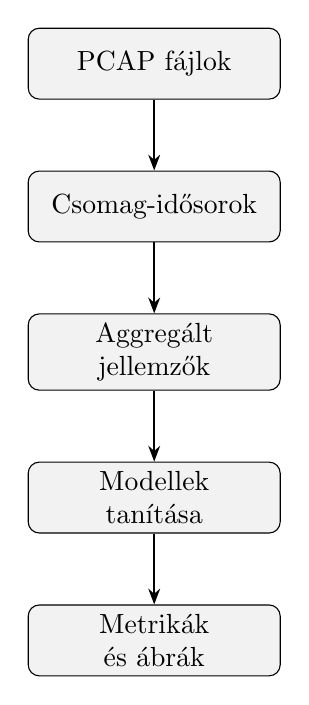
\begin{tikzpicture}[
            node distance=0.9cm,
            box/.style={draw, rounded corners, align=center, minimum width=3.2cm, minimum height=0.9cm, fill=gray!10},
            arrow/.style={-{Stealth[length=2mm]}, thick}
        ]
            \node[box] (pcap) {PCAP fájlok};
\node[box, below=of pcap] (series) {Csomag-idősorok};
            \node[box, below=of series] (features) {Aggregált\\jellemzők};
            \node[box, below=of features] (models) {Modellek\\tanítása};
\node[box, below=of models] (metrics) {Metrikák\\és ábrák};
            \draw[arrow] (pcap) -- (series);
            \draw[arrow] (series) -- (features);
            \draw[arrow] (features) -- (models);
\draw[arrow] (models) -- (metrics);
        \end{tikzpicture}
    \caption{A feldolgozási lánc fő lépései a nyers PCAP fájloktól az eredmények vizualizációjáig.}
    \label{fig:pipeline_overview}
\end{figure}

\begin{table}[tbp]
    \caption{Az aggregált folyamjellemzők főbb csoportjai és példái.}
    \vspace{2mm}
    \centering
    \begin{tabular}{p{4.5cm} p{10cm}}
        \toprule
        \textbf{Csoport} & \textbf{Jellemzők (példák)} \\ \midrule
        Csomagszámok & pl.
\texttt{total\_packets}, \texttt{in\_out\_packet\_ratio} \\
        Bájtstatisztikák & pl.
\texttt{total\_bytes}, \texttt{incoming\_bytes} \\
        Időköz-statisztikák & pl.
\texttt{mean\_inter\_arrival}, \texttt{p90\_inter\_arrival} \\
        Méretstatisztikák (összes) & pl.
\texttt{max\_packet\_size}, \texttt{mean\_packet\_size} \\
        Méretstatisztikák (irány) & pl.
\texttt{incoming\_mean\_packet\_size}, \texttt{outgoing\_std\_packet\_size} \\
        Időtartam és dinamika & pl.
\texttt{duration}, \texttt{direction\_changes} \\
        \bottomrule
    \end{tabular}
    \label{tab:feature_groups}
\end{table}

\subsection{Modellek és kiértékelés}

\textbf{Random Forest (RF).} A klasszikus gépi tanulási modell 300 döntési fát alkalmaz; ez az érték irodalmi ajánlásokkal \cite{breiman2001} összhangban biztosít megfelelő egyensúlyt a variancia-csökkentés és a számítási költség között.
A stabilizált top-10 jellemzőkiválasztás mellett, a robusztus kiértékelés érdekében a betanítás és tesztelés három különböző véletlen indítóértékkel (random seed) történik.
A modell teljesítményének statisztikai megbízhatóságát a három független futás eredményeiből számított átlag és szórás biztosítja. \newline
\textbf{Triplet MLP + KNN (DL).} A mélytanulási architektúra egy többrétegű perceptronból (MLP) áll, amely egy 32 dimenziós beágyazási teret (embedding space) tanul.
A hálózat optimalizálása Triplet Margin Loss hibafüggvénnyel történik \cite{hoffer2015}, amely arra kényszeríti a modellt, hogy az azonos osztályba (weboldalhoz) tartozó minták távolsága a beágyazási térben minimális, míg a különböző osztályoké maximális legyen.
A végső osztályozás az így kinyert beágyazásokon egy $k=5$ paraméterű k-legközelebbi szomszéd (KNN) algoritmussal történik; a $k=5$ értéket kísérleti keresztvalidáció alapján választottuk, amely a kisebb mintaszámú osztályok esetén is stabil döntési határt biztosít. \newline
\textbf{Jellemzőkiválasztási módok.} A kiértékelés során kétféle stratégia kerül alkalmazásra. A \textit{shared} beállítás esetén minden vizsgálati forgatókönyv az adott véletlen indítóértékhez (seed) tartozó, összevont adathalmazon számított kölcsönös információ (mutual information) alapján meghatározott top-10 listát használja.
Az \textit{optimized} beállítás ezzel szemben forgatókönyvenként (pl. baseline, obfs4) dedikált top-10 jellemzőkészletet állít elő;
ehhez az RF több futásból stabilizált fontossági rangsort, a DL modell pedig mutual information metrikát alkalmaz.
A zero-shot kiértékelés során a betanítás a baseline adatokon, míg a tesztelés az obfs4 adatokon történik; az eredmények az ismételt futások átlagát és szórását mutatják (átlag $\pm$ szórás), és a \ref{tab:results_closed_world}. és \ref{tab:results_open_world}. táblázatokban kerülnek összesítésre.
\subsection{Kiértékelési metrikák}

A modellek teljesítményének mérése elsősorban az osztályozási pontosság (accuracy) és a macro-F1 metrikák alapján történik.
A pontosság a helyesen besorolt minták arányát mutatja a teljes adathalmazon, míg a macro-F1 az egyes osztályokon külön-külön kiszámított F1-pontszámok számtani átlaga:
\begin{equation}
    \mathrm{Acc} = \frac{1}{N} \sum_{i=1}^{N} \mathbf{1}[\hat{y}_i = y_i], \quad
    \mathrm{MacroF1} = \frac{1}{C} \sum_{c=1}^{C} \mathrm{F1}_c,
\end{equation}
ahol $N$ az összes minta száma, $C$ az osztályok száma, $y_i$ és $\hat{y}_i$ pedig a valós, illetve a modell által prediktált címke.
Nyílt világú (open-world) beállítás esetén külön kiértékelésre kerül az ``Other'' kategória visszahívási (recall) értéke is.
Ennek vizsgálata azért kritikus, mert ez a metrika számszerűsíti, hogy az alkalmazott modell milyen hatékonysággal képes az ismeretlen forgalmat leválasztani az előre ismert, zárt világú osztályokról.
\subsection{Ábrák és vizuális összegzés}
Az ábrák a mentett metrikákból automatikusan készülnek, ezért az ábrák
és a táblázatok ugyanabból a kiértékelési kimenetből készülnek.
Az ábrák
célja, hogy a fő trendeket gyorsan összegezze, majd részletesebb bontást
adjon beállítás, jellemzőkiválasztási mód és osztályszintű viselkedés
szerint.
A zárt világú összegzést a \ref{fig:closed_world_summary}. ábra mutatja.
A \textit{shared} és \textit{optimized} beállítások különbségeit a
\ref{fig:shared_vs_optimized_delta}. ábra emeli ki, a nyílt világú
beállítások közti eltéréseket pedig a \ref{fig:open_world_focus}.
ábra foglalja össze.
A jellemzőkiválasztás hatását és stabilitását a
\ref{fig:feature_importance_shared}. és \ref{fig:feature_importance_separate}.
ábrák szemléltetik. Az osztályszintű
viselkedést a \ref{fig:confusion_matrices_recall}. ábra
konfúziós mátrixai, az
ismeretlen forgalom elkülönítését pedig a \ref{fig:other_recall_open_world}.
ábra jelzi.
\begin{figure}[tbp]
    \centering
    \includegraphics[width=0.92\linewidth]{../figures/01_closed_world_summary.pdf}
    \caption{Zárt világú teljesítmény-összegzés a két modellre.}
    \label{fig:closed_world_summary}
\end{figure}

\begin{figure}[tbp]
    \centering
    \includegraphics[width=0.92\linewidth]{../figures/03_shared_vs_optimized_delta.pdf}
    \caption{A \textit{shared} és \textit{optimized} beállítások közti különbségek (delta) pontosságban és macro-F1-ben.}
    \label{fig:shared_vs_optimized_delta}
\end{figure}

\begin{figure}[tbp]
    \centering
    \includegraphics[width=0.92\linewidth]{../figures/04_open_world_focus.pdf}
    \caption{Nyílt világú beállítások összehasonlítása.}
    \label{fig:open_world_focus}
\end{figure}

\begin{figure}[tbp]
    \centering
    \includegraphics[width=0.92\linewidth]{../figures/05_feature_importance_shared.pdf}
    \caption{A top-10 jellemzők fontossága a közös (shared) kiválasztás mellett.}
    \label{fig:feature_importance_shared}
\end{figure}

\begin{figure}[tbp]
    \centering
    \includegraphics[width=0.92\linewidth]{../figures/06_feature_importance_separate.pdf}
    \caption{Beállításonként optimalizált top-10 jellemzők összehasonlítása.}
    \label{fig:feature_importance_separate}
\end{figure}

\begin{figure}[tbp]
    \centering
    \includegraphics[width=\linewidth]{../figures/08_confusion_matrices_recall.pdf}
    \caption{Recall-normalizált konfúziós mátrixok a főbb beállításokban (shared beállítás, seed=42).}
    \label{fig:confusion_matrices_recall}
\end{figure}

\begin{figure}[hbp]
    \centering
    \includegraphics[width=0.85\linewidth]{../figures/09_other_recall_open_world.pdf}
    \caption{Az ``Other'' osztály recall értékei a nyílt világú beállításokban.}
    \label{fig:other_recall_open_world}
\end{figure}
\subsection{Reprodukálhatóság és futtatás}

Mivel az adatfeldolgozási lánc elméleti lépéseit a korábbi szakaszok már tárgyalták, ez a rész a szoftveres reprodukálhatóságot biztosító elemekre szorítkozik.
A teljes futtatási környezet, a Python függőségek (dependencies), valamint a projekt könyvtárszerkezetének részletes leírása a mellékelt \texttt{README} dokumentációban található.
A leadott laboratóriumi anyagok magukban foglalják a teljes forráskódot, a rögzített PCAP állományokat, a kinyert jellemzőket tartalmazó fájlokat, valamint a kiértékelési metrikákat és a vizualizációkat.
Ennek köszönhetően a bemutatott mérések és ábragenerálási folyamatok külső beavatkozás nélkül, teljes egészében újrafuttathatók.
\subsection{Eredmények}

A zárt világú kiértékelések eredményeit a \ref{tab:results_closed_world}. táblázat, a nyílt világú beállítások (Open-World) mérőszámait pedig a \ref{tab:results_open_world}. táblázat összesíti.
A dokumentumban bemutatásra kerülő vizualizációk (\ref{fig:closed_world_summary}. ábra) numerikus alapját teljes egészében ezek a mérések adják.
\begin{table}[tbp]
    \caption{Zárt világú (Standard) beállítások eredményei.}
    \label{tab:results_closed_world}
    \vspace{2mm}
    \centering
    \begin{tabular}{lcccc}
        \toprule
        \textbf{Beállítás} & \textbf{RF Acc.} & \textbf{RF Macro-F1} & \textbf{DL Acc.} & \textbf{DL Macro-F1} \\ \midrule
        Baseline & 80.44$\pm$0.96 & 79.76$\pm$0.99 & 61.19$\pm$2.22 & 60.23$\pm$2.47 \\
        Obfs4 & 73.33$\pm$1.78 & 71.88$\pm$1.57 & 50.64$\pm$2.59 & 49.48$\pm$2.70 \\
        Zero-Shot & 15.08$\pm$1.37 & 
10.83$\pm$1.57 & 23.01$\pm$2.59 & 18.54$\pm$2.64 \\
        \bottomrule
    \end{tabular}
\end{table}

\begin{table}[tbp]
    \caption{Nyílt világú (Open-World) beállítások eredményei.}
    \label{tab:results_open_world}
    \vspace{2mm}
    \centering
    \begin{tabular}{lcccc}
        \toprule
        \textbf{Beállítás} & \textbf{RF Acc.} & \textbf{RF Macro-F1} & \textbf{DL Acc.} & \textbf{DL Macro-F1} \\ \midrule
        OW-Baseline & 80.93$\pm$0.84 & 79.11$\pm$0.68 & 62.00$\pm$1.32 & 60.37$\pm$0.76 \\
        OW-Obfs4 & 74.10$\pm$1.59 & 
71.03$\pm$1.65 & 48.90$\pm$2.58 & 48.46$\pm$1.78 \\
        OW-Zero-Shot & 22.73$\pm$1.79 & 10.41$\pm$1.00 & 27.27$\pm$1.79 & 18.42$\pm$0.41 \\
        \bottomrule
    \end{tabular}
\end{table}

\subsection{Elemzés és megvitatás}
A kapott eredmények alapján a Random Forest algoritmus a zárt világú baseline és obfs4 beállításokban egyértelműen magasabb pontosságot és macro-F1 értéket ér el, ami a kézzel tervezett (hand-crafted) aggregált jellemzők hatékony reprezentációs képességét igazolja (lásd a \ref{fig:closed_world_summary}.
ábrát, valamint a \ref{tab:results_closed_world}. táblázatot). A zero-shot forgatókönyv esetén mindkét modell teljesítménye drasztikus degradációt szenved el a normál környezethez képest, ami a baseline és az obfs4 forgalom közötti eloszlás-eltolódás (domain shift) erőteljes gyakorlati hatására mutat rá (lásd a \ref{fig:open_world_focus}. ábrát).
Érdekesség ugyanakkor, hogy a nyílt világú zero-shot pontosság magasabb (RF: 22,73\%, DL: 27,27\%), mint a zárt világú (RF: 15,08\%, DL: 23,01\%).
Ez a látszólagos javulás nem a modellek robusztusságából fakad, hanem a nyílt világú tesztkörnyezet sajátosságának a következménye: a modellek az ismeretlen (,,Other") osztályra rendkívül magas visszahívási (recall) értéket érnek el (lásd a \ref{fig:other_recall_open_world}. ábrát), ami az osztály mintaeloszlása miatt mesterségesen megemeli az összesített pontosságot, miközben a macro-F1 értékek elhanyagolható szinten maradnak (RF: 10,41\%, DL: 18,42\%). A Triplet MLP ugyanakkor számottevően stabilabb zero-shot teljesítményt nyújt (Zárt világú Zero-Shot: DL 23,01\% vs. RF 15,08\%), ami a tanult beágyazási tér robusztusabb általánosítási képességére utal. 

Bár az \textit{optimized} jellemzőkiválasztási beállítás több esetben kismértékű javulást eredményez, ez az előny nem konzisztens. Emiatt a \textit{shared} beállítás 
optimális kompromisszumot biztosít a modellek összehasonlíthatósága és a prediktív teljesítmény között (lásd az \ref{fig:shared_vs_optimized_delta}. ábrát). A top-10 lista stabilitása azt bizonyítja, hogy a leginformatívabb aggregált jellemzők robusztusak a tanító- és teszthalmaz véletlenszerű felosztásával szemben. A nyílt világú beállításokban a visszahívásra (recall) normalizált konfúziós mátrixok jól szemléltetik, hogy a modellek az ``Other'' kategóriát többnyire sikeresen különítik el a zárt világú osztályoktól, ugyanakkor ez a magas felismerési arány gyakran a precízió (precision) rovására történik (lásd a \ref{fig:confusion_matrices_recall}. és \ref{fig:other_recall_open_world}. ábrát).
\subsection{Korlátok}
A mérési módszertan és a kiértékelés az alábbi korlátokkal rendelkezik:
\begin{itemize}
    \item A vizsgálat kizárólag aggregált folyamjellemzőkre épül, ami az eredeti csomag-idősorok finom dinamikai mintázatainak elvesztésével járhat. Ez különösen a zero-shot forgatókönyvben érezteti hatását: a \ref{fig:confusion_matrices_recall}. ábrán látható, hogy obfs4 forgalmon tesztelve az osztályszintű visszahívás számos webhelynél közel nullára esik, ami arra utal, hogy az aggregált statisztikák nem képesek megőrizni a két forgalomtípus közötti finomabb időbeli mintázatokat.
\item Mivel a nyílt világú ``Other'' osztály rendkívül heterogén (ismeretlen weboldalak sokaságának forgalmát aggregálja), a modellek számára komoly kihívást jelent ennek éles határvonalú elkülönítése a prediktálható, zárt világú osztályoktól, ami törvényszerűen a precíziós mutatók csökkenését eredményezi. A \ref{fig:other_recall_open_world}. ábrán jól látható, hogy a magas visszahívási értékeket (RF OW-Baseline: 96,9\%) jellemzően alacsony precízió kíséri, mivel a modellek az ismeretlen forgalom egy részét tévesen az ``Other'' kategóriába sorolják.
\item A radikális dimenziócsökkentés (kizárólag a top-10 jellemző statikus megtartása a 21 dimenziós teljes jellemzőtérből) következtében a ritkábban előforduló, ám egy-egy osztály esetében lokálisan informatív mintázatok prediktív ereje elveszhet. A \ref{fig:shared_vs_optimized_delta}. ábrán megfigyelhető, hogy az \textit{optimized} kiválasztás egyes beállításokban akár 4--6 százalékpontos macro-F1 javulást is eredményez a \textit{shared} beállításhoz képest, ami azt jelzi, hogy a top-10-es korlát szűkíti a reprezentációs kapacitást.
\end{itemize}

\subsection{Következtetések és jövőbeli munka}
\label{sec:kovetkeztetesek}

A projekt igazolja, hogy a klasszikus és a mélytanulás-alapú modellek eltérő erősségekkel rendelkeznek a Tor hálózaton végzett WF támadások vizsgálatában.
Míg a Random Forest algoritmus a baseline környezetben magasabb osztályozási pontosságot ér el, addig a Triplet MLP architektúra a zero-shot forgatókönyvek során bizonyul robusztusabbnak, és jobban általánosít az ismeretlen környezetekre.
Mivel a hálózati forgalom statisztikai eloszlása időben változik -- ezt a jelenséget \textit{concept drift}-nek nevezzük, utalva arra, hogy a tanítóadatok és a jövőbeli minták eloszlása fokozatosan eltolódhat -- a jövőbeli kutatások során érdemes több időszakból és mindkét adatkörnyezetből (baseline, obfs4) kiterjedtebb tanítóadat-halmazt gyűjteni, majd a modelleket egy időben elkülönített (time-separated) teszthalmazon kiértékelni.
Ezt a megközelítést kiegészítheti a modellek friss mintákon történő periodikus újratanítása, valamint a komplexebb idősoros jellemzők (nyers csomag-idősorok, burst-mintázatok, n-gram vagy reprezentáció-tanuláson alapuló leírások) bevonása.
Végül indokolt a modellfrissítés költséghatékonyságának számszerűsítése is: vizsgálni kell, hogy mennyi új adat és számítási kapacitás szükséges egy adott teljesítménynövekedés eléréséhez, illetve milyen frissítési gyakoriság biztosítja az optimális kompromisszumot.
\subsection{Összefoglalás}
\label{sec:osszefoglalas}

A laboratóriumi munka során egy teljes mértékben reprodukálható WF adatfeldolgozási lánc (pipeline) került kialakításra, amely a nyers PCAP állományok kinyerésétől a kiértékelési metrikák kiszámításáig és az eredmények vizualizációjáig biztosít egy egységes, automatizált keretrendszert.
A végrehajtott kísérletek rámutattak, hogy a Random Forest algoritmus a baseline és az obfs4 környezetekben magasabb osztályozási pontosságot ér el, míg a Triplet MLP architektúra a zero-shot beállítások esetén robusztusabb általánosítási képességgel rendelkezik.
A nyílt világú vizsgálatok igazolták, hogy az ismeretlen forgalmat aggregáló ``Other'' osztály leválasztása lehetséges, azonban ennek precíziója jelenleg korlátos.
A mérések legfőbb tanulsága, hogy a baseline és az obfs4 forgalom statisztikai eloszlása szignifikánsan eltér (domain shift).
Ennek feloldása érdekében a jövőbeli kutatások fókuszába a heterogén környezetekből származó adatokon betanított modellek, valamint a mélyebb, idősoros forgalmi mintázatok vizsgálata kell, hogy kerüljön (lásd még a \textit{concept drift} jelenségét a~\ref{sec:kovetkeztetesek}. szakaszban).
\newpage

%==================================================================
\section{Irodalom és csatlakozó dokumentumok jegyzéke}
\label{sec:irod-es-csatl}
 
\label{sec:tanulm-irod-jegyz}
 
\begin{thebibliography}{9}
 
\bibitem{dingledine2004} R. Dingledine, N. Mathewson, and P. Syverson,
``Tor: The Second-Generation Onion Router,''
in \textit{Proc.
13th USENIX Security Symposium (USENIX Security '04)},
San Diego, CA, USA, 2004, pp. 303--320.
[Online].
Elérhető: \url{https://www.usenix.org/conference/13th-usenix-security-symposium/tor-second-generation-onion-router}
(Letöltve: 2026. május 20.)
 
\bibitem{cherubin2022} G. Cherubin, R. Jansen, and C. Troncoso,
``Online Website Fingerprinting: Evaluating Website Fingerprinting Attacks on Tor in the Real World,''
in \textit{Proc.
31st USENIX Security Symposium (USENIX Security '22)},
2022, pp. 753--770.
[Online].
Elérhető: \url{https://www.usenix.org/conference/usenixsecurity22/presentation/cherubin}
(Letöltve: 2026. május 20.)
 
\bibitem{sirinam2018} P. Sirinam, M. Imani, M. Juarez, and M. Wright,
``Deep Fingerprinting: Undermining Website Fingerprinting Defenses with Deep Learning,''
in \textit{Proc.
2018 ACM SIGSAC Conf. Computer and Communications Security (CCS '18)},
Toronto, ON, Canada, 2018, pp. 1928--1943.
DOI: \url{https://doi.org/10.1145/3243734.3243768}
(Letöltve: 2026. május 20.)
 
\bibitem{wiley2013obfs4} Y. Angel (The Tor Project),
``obfs4: The obfourscator,''
Tor Project, 2014.
[Online].
Elérhető: \url{https://gitlab.com/yawning/obfs4}
(Letöltve: 2026. május 20.)
 
\bibitem{breiman2001} L. Breiman,
``Random Forests,''
\textit{Machine Learning}, vol. 45, no.
1, pp. 5--32, 2001.
DOI: \url{https://doi.org/10.1023/A:1010933404324}
(Letöltve: 2026. május 20.)

\bibitem{hoffer2015} E. Hoffer and N. Ailon,
``Deep Metric Learning Using Triplet Network,''
in \emph{Similarity-Based Pattern Recognition}, 2015, pp. 84--92.
DOI: \url{https://doi.org/10.1007/978-3-319-24261-3_7}.
(Letöltve: 2026. május 20.)

\end{thebibliography}

%==================================================================
\subsection{A csatlakozó dokumentumok jegyzéke}
\label{sec:csat-irod}

A projekt reprodukálásához szükséges teljes forráskód, az adatgyűjtési környezet és a dokumentáció elérhető a publikus GitHub repozitóriumban:
\begin{itemize}
    \item[] \textbf{Pálos Ferenc: \textit{Tor Website Fingerprinting Pipeline}} \\
    Elérhető: \url{https://github.com/palosferi/onlab}
\end{itemize}

A beadott csatlakozó anyagok a projekt lokális könyvtárában az alábbi struktúra szerint találhatók:
\begin{itemize}
    \item \texttt{src/} -- A feldolgozási és kiértékelési pipeline implementációja.
\item \texttt{scripts/collection/} -- Az automatizált adatgyűjtést végző szkriptek.
    \item \texttt{figures/} -- A kiértékelés során keletkezett nyers JSON metrikák és a generált ábrák.
\item \texttt{tor\_dataset/} -- A mérések alapjául szolgáló nyers PCAP állományok.
    \item \texttt{irasbeli\_beszamolo/figs/} -- A beszámoló fordításához szükséges lokális ábrák.
\end{itemize}

\end{document}

%%% Local Variables: 
%%% mode: latex 
%%% TeX-master: t 
%%% End: